\documentclass[11pt]{exam}
\usepackage{amsmath}
\usepackage{amsthm}
\usepackage{amssymb}
\newcommand{\myname}{Cael Howard} %Write your name in here
\newcommand{\myUCO}{cthoward} 
\newcommand{\myhwtype}{Homework}
\newcommand{\myhwnum}{4} %Homework set number
\newcommand{\myclass}{Compsci 166}
\newcommand{\mylecture}{}
\newcommand{\mysection}{}

% Prefix for numedquestion's
\newcommand{\questiontype}{Question}


% Use this if your "written" questions are all under one section
% For example, if the homework handout has Section 5: Written Questions
% and all questions are 5.1, 5.2, 5.3, etc. set this to 5
% Use for 0 no prefix. Redefine as needed per-question.
\newcommand{\writtensection}{0}

\usepackage{amsmath, amsfonts, amsthm, amssymb}  % Some math symbols
\usepackage{enumerate}
\usepackage{enumitem}
\usepackage{graphicx}
\usepackage{hyperref}
\usepackage[all]{xy}
\usepackage{wrapfig}
\usepackage{fancyvrb}
\usepackage[T1]{fontenc}
\usepackage{listings}
\usepackage{accents}
\usepackage{braket}
\usepackage{tikz}
\usepackage{quantikz}
\usepackage{commath}

\usepackage{centernot}
\usepackage{mathtools}
\DeclarePairedDelimiter{\ceil}{\lceil}{\rceil}
\DeclarePairedDelimiter{\floor}{\lfloor}{\rfloor}
\DeclarePairedDelimiter{\card}{\vert}{\vert}


\setlength{\parindent}{0pt}
\setlength{\parskip}{5pt plus 1pt}
\pagestyle{empty}

\def\indented#1{\list{}{}\item[]}
\let\indented=\endlist

\newcounter{questionCounter}
\newcounter{partCounter}[questionCounter]

\newenvironment{namedquestion}[1][\arabic{questionCounter}]{%
    \addtocounter{questionCounter}{1}%
    \setcounter{partCounter}{0}%
    \vspace{.2in}%
        \noindent{\bf #1}%
    \vspace{0.3em} \hrule \vspace{.1in}%
}{}

\newenvironment{numedquestion}[0]{%
	\stepcounter{questionCounter}%
    \vspace{.2in}%
        \ifx\writtensection\undefined
        \noindent{\bf \questiontype \; \arabic{questionCounter}. }%
        \else
          \if\writtensection0
          \noindent{\bf \questiontype \; \arabic{questionCounter}. }%
          \else
          \noindent{\bf \questiontype \; \writtensection.\arabic{questionCounter} }%
        \fi
    \vspace{0.3em} \hrule \vspace{.1in}%
}{}

\newenvironment{alphaparts}[0]{%
  \begin{enumerate}[label=\textbf{(\alph*)}]
}{\end{enumerate}}

\newenvironment{arabicparts}[0]{%
  \begin{enumerate}[label=\textbf{\arabic{questionCounter}.\arabic*})]
}{\end{enumerate}}

\newenvironment{questionpart}[0]{%
  \item
}{}

\newcommand{\bravec}[2]{\begin{bmatrix} #1 & #2 \end{bmatrix}}

\newcommand{\ketvec}[2]{\begin{bmatrix} #1 \\ #2 \end{bmatrix}}
\newcommand{\transgate}[4]{\begin{bmatrix} #1 & #2\\ #3 & #4 \end{bmatrix}}

\newcommand{\hgate}[0]{$\transgate{1/\sqrt{2}}{1/\sqrt{2}}{1/\sqrt{2}}{-1/\sqrt{2}}$}
\newcommand{\xgate}{$\transgate{0}{1}{1}{0}$}
\newcommand{\cgate}{$\transgate{1}{0}{0}{i}$}
\newcommand{\zgate}{$\transgate{1}{0}{0}{-1}$}

\newcommand{\answerbox}[1]{
\begin{framed}
\vspace{#1}
\end{framed}}

\pagestyle{head}

\headrule
\header{\textbf{\myclass\ \mylecture\mysection}}%
{\textbf{\myname\ (\myUCO)}}%
{\textbf{\myhwtype\ \myhwnum}}

\begin{document}
\thispagestyle{plain}
\begin{center}
  {\Large \myclass{} \myhwtype{} \myhwnum} \\
  \myname{} (\myUCO{}) \\
  \today
\end{center}


%Here you can enter answers to homework questions

\begin{numedquestion}
    \textbf{1)} What is your guess on the winning probability for this strategy?

    \textbf{Answer:}\\
    The strategy seems to result in a winning probability of $1/2$.
    \vspace{1em}

    \textbf{2)} Conisder the case where $x=0$ and $y=1$. Let's suppose that Bob measures first for our analysis. What are the possible states after Bob's measurement?

    \textbf{Answer:}\\
    If both players receive a $1$, Bob measures $\ket{0}$ with probability $1/2$ and $\ket{1}$ with probability $1/2$.
    \vspace{1em}

    \textbf{3)} For each case, Alice measures the same quibit as Bob with probability $1$.
    \vspace{1em}

    \textbf{4)} The probability that Alice and Bob win using this strategy is $1$.
    \vspace{1em}

    \textbf{5)} Bob measures $\ket{+}$ and $\ket{-}$ with probability $1/2$ for each case.
    \vspace{1em}

    \textbf{6)} For each case, Alice measures $\ket{0}$ and $\ket{1}$ with probability $1/2$.
    \vspace{1em}

    \textbf{7)} The probability that Alice and Bob win using this strategy is $1/2$ as they need to output the same bit.
    \vspace{1em}

    \textbf{8)} If all four input pairs occur uniformly, the probability that Alice and Bob win the game is $1/2$.
\end{numedquestion}

\begin{numedquestion}
    \textbf{1)} A classical strategy that allows for a win rate of $3/4$ would be to fix one individual to output a $1$ and the others to output $0$. This results in an odd number of $1$'s being output which leads to them winning $3/4$ths of the time. 
    \vspace{1em}

    \textbf{2)} If all individuals are given $1$, after the first individual measures their quibit, it collapses to the following positions.
    \begin{align*}
    \ket{0}: \frac{1}{\sqrt{2}} (\ket{00} - \ket{11})\\
    \ket{1}: \frac{1}{\sqrt{2}} (-\ket{01} - \ket{10})
    \end{align*}
    In both of these cases, the total number of $1$'s is even, meaning that they win with probability $1$.
    \vspace{2em}

    \textbf{3)} Consider the case where Alice gets a $1$. The quibit collapses to the following:
    \begin{align*}
    \ket{0}:&\frac{1}{\sqrt{2}}(\ket{++} - \ket{--})\\
    & \frac{1}{\sqrt{2}}(\frac{1}{2}(\ket{00} + \ket{10} + \ket{01} + \ket{11}) - \frac{1}{2}(\ket{00} - \ket{01} - \ket{10} + \ket{11}))\\
    & \frac{1}{\sqrt{2}}(\ket{10} + \ket{01})\\
    \ket{1}:&\frac{1}{\sqrt{2}}(\ket{+-} + \ket{-+})\\
    & \frac{1}{\sqrt{2}}(\ket{00} - \ket{01} + \ket{10} - \ket{11}) + \frac{1}{\sqrt{2}} (\ket{00} - \ket{10} + \ket{01} - \ket{11})\\
    &\frac{1}{\sqrt{2}}(\ket{00} - \ket{11})
    \end{align*}
    For both cases, since the total number of 1's is odd, they win with probability 1.
\end{numedquestion}

\begin{numedquestion}
    \textbf{1)} A great strategy would be to give both bits to the frogs and output whatever they tell you to.
    \vspace{1em}

    \textbf{2)} $X \cdot Y = 3 \text{ mod } 2 = 1$
    \vspace{1em}

    \textbf{3)} If both players send the other their $n$ bits, they can each calculate $X \cdot Y$ locally and output the answer.
    \vspace{1em}

    \textbf{4)} A strategy where both players send one bit to the other and can deduce the correct inner product is as follows. They send the other individual a $1$ if their frog output an odd amount of 1's, else they send a $0$. Now, if there are an even amount of $1$'s, they know that the inner product is $0$. Else, they know that there are an odd number.

    \textbf{6)} A strategy do derive the result of a function is similar. The cardinality of the number of $1$'s and $0$'s can be used to determine the cardinality of the result. Therefore, the mod 2 of that result can be deduced.
\end{numedquestion}

\newpage
\begin{numedquestion}
    \textbf{1)}
    \begin{tabular}{|l|c|}
        \hline
        Input & Output \\
        \hline
        000 & 000\\
        001 & 001\\
        010 & 010 \\
        011 & 011 \\
        100 & 100 \\
        101 & 101 \\
        110 & 111 \\
        111 & 110 \\
        \hline
    \end{tabular}
    \vspace{1em}

    \textbf{2)}
    \begin{center}
        \begin{quantikz}
        \ket{a} & \qw & \ctrl{1} & \qw\\
        \ket{b} & \qw & \ctrl{1} & \qw\\
        \ket{c} & \qw & \targ{} & \qw\\
        \end{quantikz}
    \end{center}

    \begin{center}
        \begin{quantikz}
        \ket{a} & \qw & \targ{} & \qw\\
        \ket{1} & \qw & \ctrl{-1} & \qw\\
        \ket{1} & \qw & \ctrl{-1} & \qw\\
        \end{quantikz}
    \end{center}
    \vspace{1em}

    \textbf{3)}
    \begin{figure}[h]
        \centering
        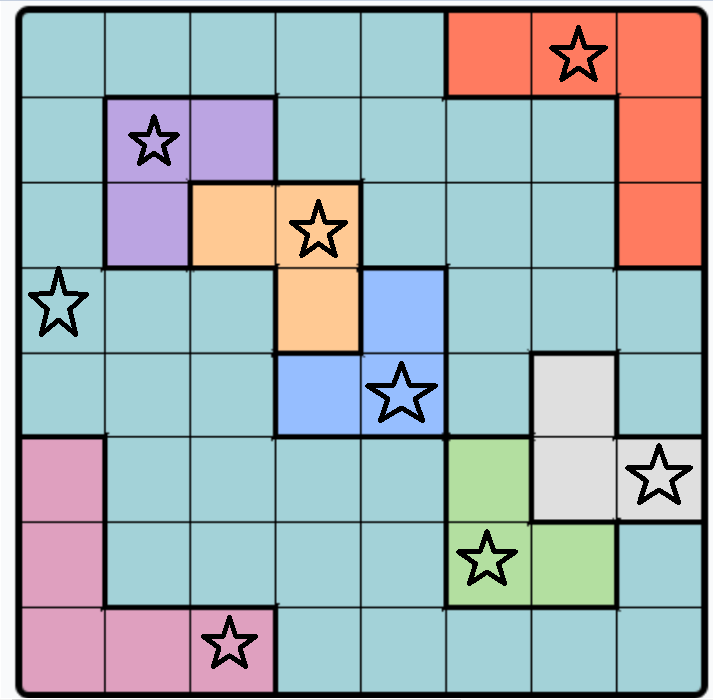
\includegraphics[width=0.4\textwidth]{img/cs166q4.png}
    \end{figure}
    \newpage
    \textbf{4)} Queens is in NP since it can be checked in polynomial time by making sure all rows/columns have 1 queen.
    \vspace{1em}
    
    \textbf{5)} Collatz is in NP as we assume that any sequence either repeats or reaches 1 in polynomial time. Therefore, running the algorithm will give the answer to whether or not it it or is not in the language.
\end{numedquestion}

\end{document}
